\section{Evaluation} \label{eval}
In this section, we evaluate the performance of \sys based on the RDMA test tools and real applications. We expect to answer the following questions: 1) How does the performance of \sys compared to that of \native for both VMs and containers? 2) How about the scalability of \sys? 3) Can \sys be adapted to the real-world RDMA applications in both VMs or containers?
%
%\begin{itemize}
%\item How does the performance of \sys compared to that of \native for both VMs and containers?
%\item How about the scalability of \sys?
%\item Can \sys be adapted to the real-world RDMA applications in both VMs or containers?
%
%\end{itemize}

\subsection{Experiment Methodology}


We implement the \sys system in Linux environment. The hypervisor of VM is QEMU/KVM and the container engine is Docker. The vRNIC frontends for VMs and containers are implemented differently. The \sys Core~(with vRNIC backends) includes about 2000 lines of code.
And in the management node, Zookeeper~\cite{zookeeper} is used to keep the information for RDMA resources~(such as RDMA address mappings and the numbers of VFs) and the policies~(such as QP limit and QoS).
In addition, we modified the \textit{libibverbs-41mlnx1} Verbs library, the \textit{librdma-cm} Verbs library for connection management, and the \textit{libmlx4-41mlnx1} user-space RNIC driver.
And some minor modifications are made to the host OS kernel, such as caching GPA into RNIC and mapping DoorBells.
Based on our approach, user-level applications don't need to be modified or recompiled because the RDMA APIs are not changed. %In this section, some implementation details are introduced.

All experiments are carried out on two servers. The settings mainly include three parts: host server, VMs and containers. 
Each host server is equipped with 4 Intel Xeon E7-4850 2.40GHz 16-core CPUs and 1 TB RAM. The RNIC used is Mellanox ConnectX-3 56 Gb/sec, which performs RDMA communication under Infiniband.  The operating system is CentOS 7.4.1708 (Linux 3.10.0-693.el7.x86\_64). The RDMA driver installed on the host server is Mellanox OFED 4.4-2.0.7.0~\cite{mlnx-ofed}. To keep consistence, VMs and containers are built based on the same OS images as host. All VMs are based on QEMU~(5.1.50)~\cite{qemu} enabled with KVM~\cite{kvm}. We provide 16 cores and 64 GB memory for each VM. We run containers using Docker~(18.06.1-ce)~\cite{docker} and limit the CPU and memory resources to the same settings as the VM. In addition, all the applications are compiled with GCC/G++ 4.8.5 with the O3 compilation configuration. Note that the management node is on one of two evaluated nodes in our evaluation setting. Since the management node is not involved on the data-path, it has very limited influence on the performance of one-sided or two-sided communication.


\subsection{Basic Evaluation}

Throughput and latency are the key targets of network performance. Latency is the time taken for a packet to be transferred. Throughput is the quantity of data~(some packets) to be transferred within a unit of time. RDMA supports two different data transmission modes: one-sided and two-sided. Due to the difference performance between them, we evaluate them respectively.


Based on the RDMA benchmark test tool perftest~\cite{perftest}, we evaluated the performance~(throughput and latency) of \native, hardware virtualization SR-IOV for VMs,  software virtualization for containers~(FreeFlow) and \sys in VMs or containers. SR-IOV is the hardware virtualization solution for VMs. Because VMs monopolize a PCI-e device, the SR-IOV vitualizes multiple lightweight PCI-e physical devices for diffrent VMs, which cannot used by containers. Thus, we didn't measure the performance of SR-IOV in containers. In addition, we didn't compare the performance of \sys with that of MasQ because it is not open-sourced. For one-sided write operations, we use ``ib\_write\_bw'' and ``ib\_write\_lat'' commands; for one-sided read operation, we use ``ib\_read\_bw'' and ``ib\_read\_lat'' commands. For two-sided operations~(Send and Recv), we use ``ib\_send\_bw'' and ``ib\_send\_lat'' commands. The specific process is: after the RDMA connection is established between the client and the server, the message bytes are transmitted. The message sizes are from 4B to 256KB. For each message size,  it is evaluated iteratively 1000 times and the average results are used for evaluation.  Note that we also collected the data whose message sizes are larger than 256KB, such as 512KB, 1MB and 2MB. After the message sizes are larger than 256KB, the performance slowdown for \sys is negligible. Thus, these results are not included in the corresponding figures due to the space constraint. 


\subsubsection{\textbf{Throughput}}
\
\noindent

\begin{figure}[!ht]
	\centering
	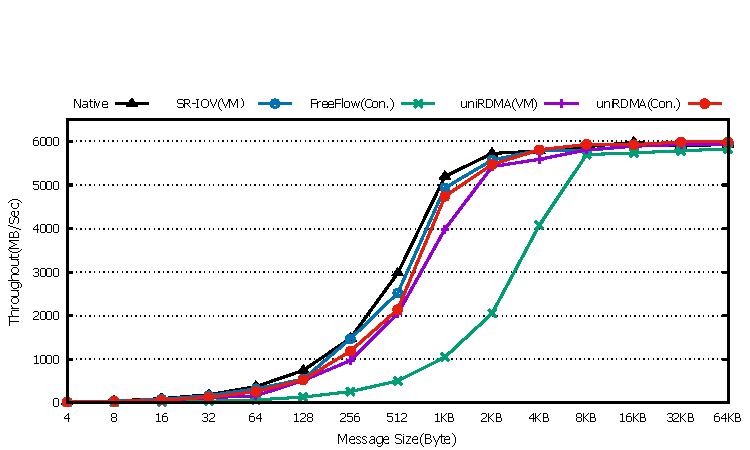
\includegraphics[width=1.00\linewidth]{images/write-bw.pdf}
	\caption{The throughout of one-sided mode.}
	\label{fig:write-bw}
\end{figure}


\begin{figure}[!ht]
	\centering
	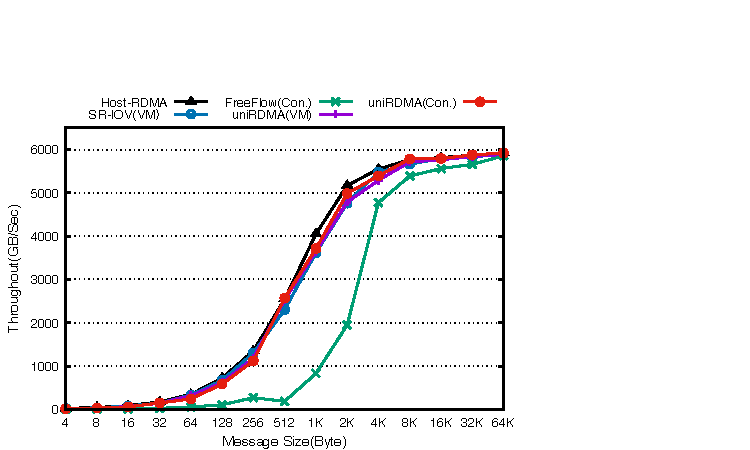
\includegraphics[width=1.00\linewidth]{images/send-bw.pdf}
	\caption{The throughout of two-sided mode.}
	\label{fig:send-bw}
\end{figure}


As the data show in Figure~\ref{fig:write-bw} and Figure~\ref{fig:send-bw}, \sys can achieve comparable throughput compared with SR-IOV and \native. When the message gradually increases, such as reaching 256KB, the throughput of each framework tends to be consistent. The reason is that the bandwidth of RDMA netwrok is saturated after that. %, and the delay overhead of FreeFlow has been covered by waiting delay in RNIC.

For one-sided mode as the data in Figure~\ref{fig:write-bw} show, the average throughput of \sys in VMs has only 4$\%$ slowdown to that of SR-IOV in VMs. And the average throughput of \sys in containers has only 0.4$\%$ slowdown to that of \native. For two-sided mode as the data in Figure~\ref{fig:send-bw} show, the average throughput of \sys in VMs has only 3$\%$ slowdown to that of SR-IOV in VMs. The average throughput of \sys in containers has only 5$\%$ slowdown to that of \native.




Compared with FreeFlow, when the message is small, the throughput of \sys has reached 4-6 times that of FreeFlow. Because FreeFlow forwards all data commands to the software virtualization layer for processing and these data are copied to the RDMA hardware. Additional memory copies involve large performance overhead. In contrast, \sys maps all RDMA resources to execute data commands in the guest user space of VMs or containers. Therefore, there is no latency for data forwarding in data path.





\subsubsection{\textbf{Latency}}
\
\noindent

\begin{figure}[!ht]
	\centering
	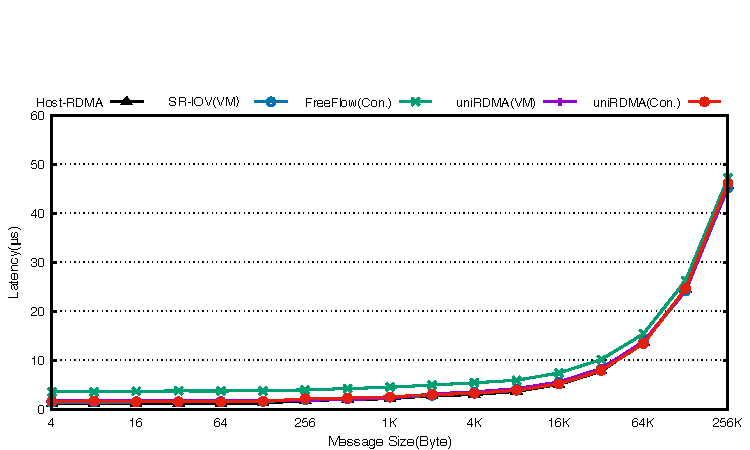
\includegraphics[width=1.00\linewidth]{images/write-lat.pdf}
	\caption{The latencty of one-sided mode.}
	\label{fig:write-lat}
\end{figure}


\begin{figure}[!ht]
	\centering
	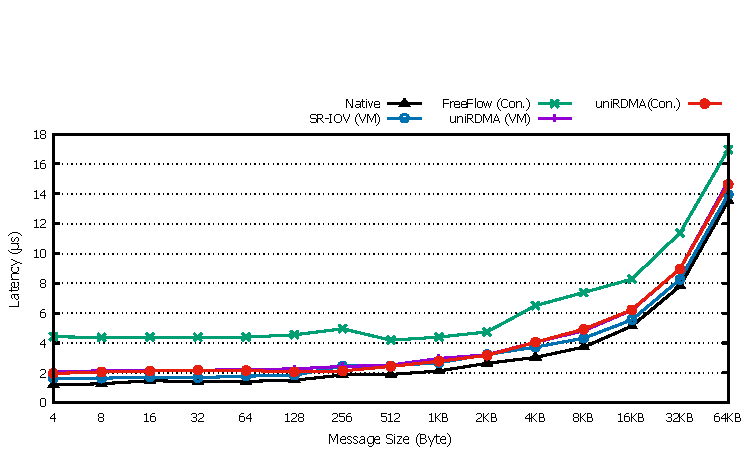
\includegraphics[width=1.00\linewidth]{images/send-lat.pdf}
	\caption{The latencty of two-sided mode.}
	\label{fig:send-lat}
\end{figure}


The latency results are shown in Figure~\ref{fig:write-lat} and Figure~\ref{fig:send-lat}. As these data show, \sys can achieve comparable letency results compared with SR-IOV and \native. The latency gradually increases as the forwarding message size becomes larger because the large message needs to be sliced into small message for network package transmission.
For one-sided mode, the latency of \sys in VMs is 4\% higher compared to that of SR-IOV in VMs. The latency of \sys in containers is about 10\% higher compared to that of \native. For two-sided mode, the latency of \sys in VMs is 0.4\% higher compared to that of SR-IOV in VMs. The latency of \sys in containers is about 10\% higher than that of \native.

Compared with FreeFlow, when the message is small, the latency of \sys is only 40\% to 60\% of FreeFlow because the overhead of additional data copy on path commands for FreeFlow involves large overhead. 





\subsection{Scalability}

With the scale of the applications and datacenter capacity rising, more and more VM instances and container instances are deployed. Thus, the scability has been a key design metric for RDMA virtualization.

To evaluate the scalability of \sys, we use aggregate throughput as the metric of scalability evaluation. It is the sum of the throughput of multiple parallel RDMA flows at the same time and has been widely used in prior works~\cite{kim2019freeflow, pfefferle2015hybrid, he2020masq}. If the aggregate throughput of multiple parallel RDMA flows is closer to the hardware throughput, the cost of RDMA virtualization is smaller, which illustrate \sys has a good scalability. The thoughput of a individual RDMA flow is fluctating at each moment and the instant RDMA throughput is difficult to align among multiple RDMA flows. Therefore, we collect and summarize the average throughput of each RDMA flow in 1 second to obtain the average aggregate throughput.

We used one-sided operation (``ib\_write\_bw'' in ~\cite{perftest}) with 2, 4, 8, 16, 32 and 64 virtual instance pairs which continuously send data (65536 Bytes) between two paris. Since the RNICs in our evaluation only supports upto 64 VFs, we use 64 instances as the maximal evaluation value.

As the data in Figure~\ref{fig:scabality} show, in the VM-only scenario, container-only scenario and hybrid scenario, the throughput of \sys is close to that of SR-IOV. The average overhead is only 1.4\%.


\begin{figure}[!ht]
	\centering
	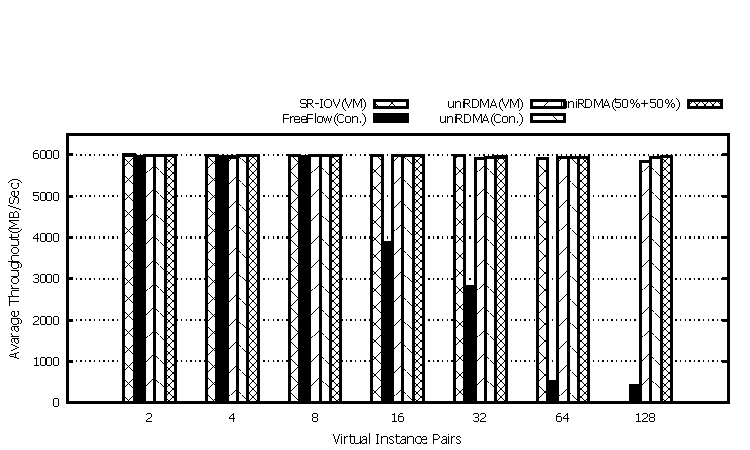
\includegraphics[width=1.0\linewidth]{images/scabality.pdf}
	\caption{\sys scalability. Aggregation throughput at different scenarios and scales are evaluated.}
	\label{fig:scabality}
\end{figure}

\subsection{Real-world Applications}

The main advantage of RDMA is about its optimized network performance in real-world applications. RDMA virtualization needs to maintain such an advantage. Therefore, we evaluate \sys and other frameworks in a RPC benchmark in rdma\_bench~\cite{rbench}. In this benchmark, UD transport with a 32-bit immediate header is used between the client and server.

\subsubsection{\textbf{RPC}}
\
\noindent



In the evaluation, the server and the client are started on two host servers. There are 16 threads for the server, and the thread number for the client is from 1, 2, 4, 8, 16 in turn. %This papers separately tested the average throughput of the server in the entire RPC process.

\begin{figure}[!ht]
	\centering
	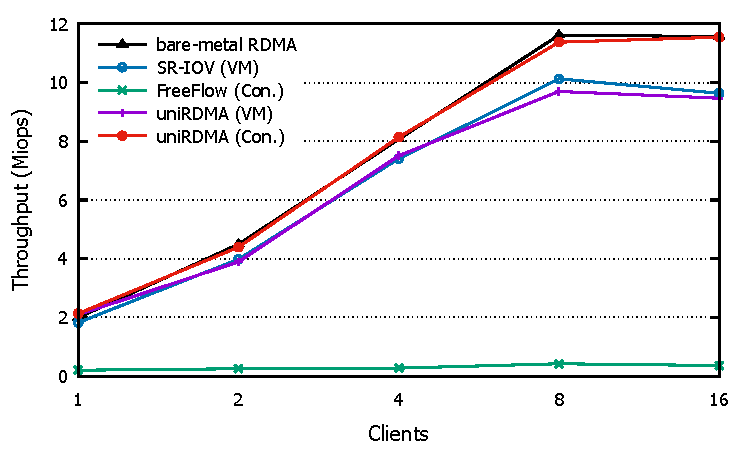
\includegraphics[width=1.0\linewidth]{images/rpc.pdf}
	\caption{The Throughput of RPC}
	\label{fig:rpc}
\end{figure}

As the data in Figure~\ref{fig:rpc} show, \sys achieves good performance for real applications. For containers, its performance is approximately the same with that of \native. For VMs, its performance is approximately the same with that of SR-IOV. In total, there is almost no performance loss. The major reason is that \sys bypasses the kernel and virtualization layer in the data path, and there is no software forwarding latency caused by virtualization. In the control path, \sys has a delay because of RDMA Verbs forwarding. However, this overhead is one-time for the RPC application and it has little influence on the overall performance. Compared with FreeFlow, the preformance \sys is better due to no additional memory copies. 



\subsubsection{\textbf{Graph500}}
\
\noindent

Graph500~\cite{Graph500} is a rating system for data intensive applications in HPC. Two banchmarks are included in Graph500. The first task is the breadth-first search~(BFS) for the graphs generated by the inpt parameters and the second one is the single source shortest path~(SSSP) for the generated graphs. 

We executed two tasks in Graph500 on two servers with 16 MPI processes. The banchmake generates graphs in the main memory with parameters scale \= 26 and edge\_factor \= 16. We run 10 times for each task and calculate the average horizontal mean of traversed edges per second (TEPS). As the data shown in Figure~\ref{fig:graph500}, the performance of \sys is very close to those of SR-IOV and \native.

\begin{figure}[!ht]
	\centering
	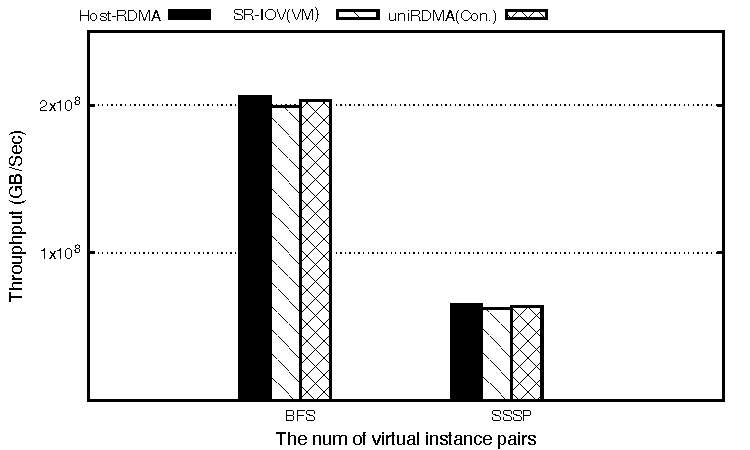
\includegraphics[width=1.0\linewidth]{images/graph500.pdf}
	\caption{The TEPS of BFS and SSSP}
	\label{fig:graph500}
\end{figure}